\documentclass[a4paper,11pt,notitlepage,fullpage]{paper}
\usepackage{fullpage}
\usepackage[utf8]{inputenc}
%\usepackage[ngerman]{babel}
\usepackage[english]{babel}
\usepackage{amsmath}
\usepackage{amssymb}
\usepackage{latexsym}
\usepackage{mathtools}
\usepackage{listings}
\usepackage{algorithm}
\usepackage{algpseudocode}
\usepackage{graphicx}
\usepackage{booktabs}
\usepackage{hhline}
\usepackage{amsthm}
\usepackage{cite}
\usepackage{wrapfig}
\usepackage{hyperref}
\usepackage{titling}
\usepackage{color}

\newcommand{\y}{\gamma}
\newcommand{\dy}{\dot\gamma}
\newcommand{\ddy}{\ddot\gamma}

\setcounter{section}{-1}
%https://tex.stackexchange.com/questions/107470/getting-section-numbering-to-start-at-0

\theoremstyle{plain}
\newtheorem{thm}{Theorem}[section] % reset theorem numbering for each chapter
\newtheorem{lem}[thm]{Lemma}
\newtheorem{col}[thm]{Corollary}
\newtheorem{defn-lem}[thm]{Definition-Lemma}

\theoremstyle{definition}
\newtheorem{defn}[thm]{Definition} % definition numbers are dependent on theorem numbers
\newtheorem{exmp}[thm]{Example} % same for example numbers
\newtheorem{obsv}[thm]{Observation}

%https://tex.stackexchange.com/questions/45817/theorem-definition-lemma-problem-numbering

\makeatletter
\newcommand*{\toccontents}{\@starttoc{toc}}
\makeatother

%https://tex.stackexchange.com/questions/296207/reducing-space-between-items-of-reference
\usepackage{etoolbox}
\patchcmd{\thebibliography}
  {\settowidth}
  {\setlength{\itemsep}{0pt plus 0.1pt}\settowidth}
  {}{}
\apptocmd{\thebibliography}
  {\footnotesize}
  {}{}

\setlength{\droptitle}{-60pt}

\begin{document}
\author{Lectured by \textsc{Univ.Prof. Dr. Ivan Izmestiev}, latexed by \textsc{Florian Bogner}}
\title{Differential Geometry}
\maketitle

\toccontents

\section{Introduction}

The course will consist of:

\begin{itemize}
\item Curves in $\mathbb R^2$ and $\mathbb R^3$

We will look at \emph{length}, \emph{curvature}, as well as \emph{torsion} for Curves in $\mathbb R^3$.

\item Surfaces

We will look at \emph{area} and \emph{curvature}. For curvature, there are two different notions:
\begin{itemize}
\item extrinsic: How much is the surface bent in different directions?
\item intrinsic: If we bend the surface without stretching and shrinking, then some ``curvedness'' remains.
\end{itemize}

\begin{figure}[H]
\centering
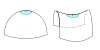
\includegraphics[width = 0.6\textwidth]{img/intrinsic-curvature}
\caption{Convex surface and saddle surface.}
\label{fig:intrinsic}
\end{figure}

The area of a disk with radius $r$ on a curved surface is different from that on an intrinsically flat surface. It is a manifestation of intrinsic surface curvature.

\begin{itemize}
\item On a convex surface the area is smaller than $\pi r^2$
\item On a saddle surface the area is bigger than $\pi r^2$
\end{itemize}


\item Riemannian Geometry

A Riemannian metric on a domain $U \subset \mathbb R^n$ is a length measurement inspired by differential geometry. There is no extrinsic curvature (bendedness) but the intrinsic curvature is present.

For example: In General Relativity a mass bends the space\footnote{Actually, the space-time is bent, and the metric is not Riemannian but Lorentzian.}, see Figure \ref{fig:gravlens}.

\begin{figure}
\centering
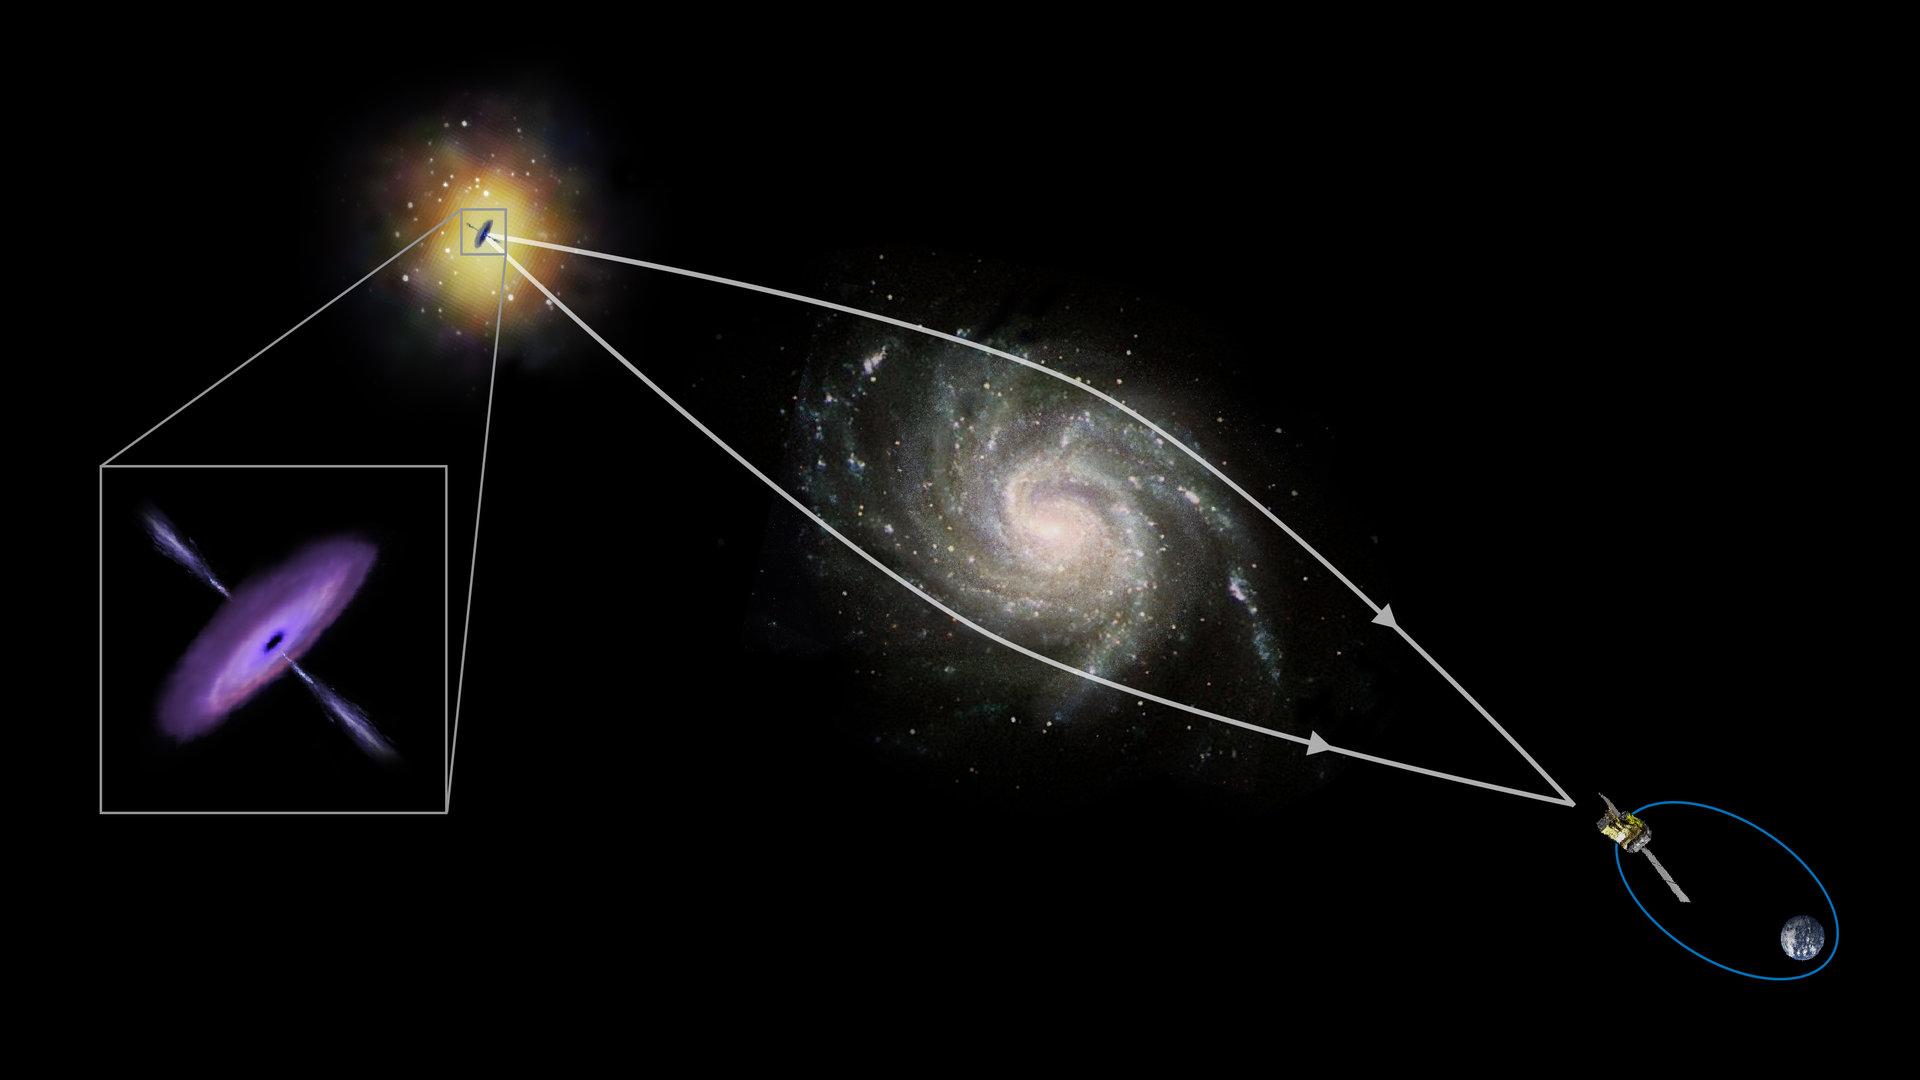
\includegraphics[width = 0.4\textwidth]{img/gravlens1}
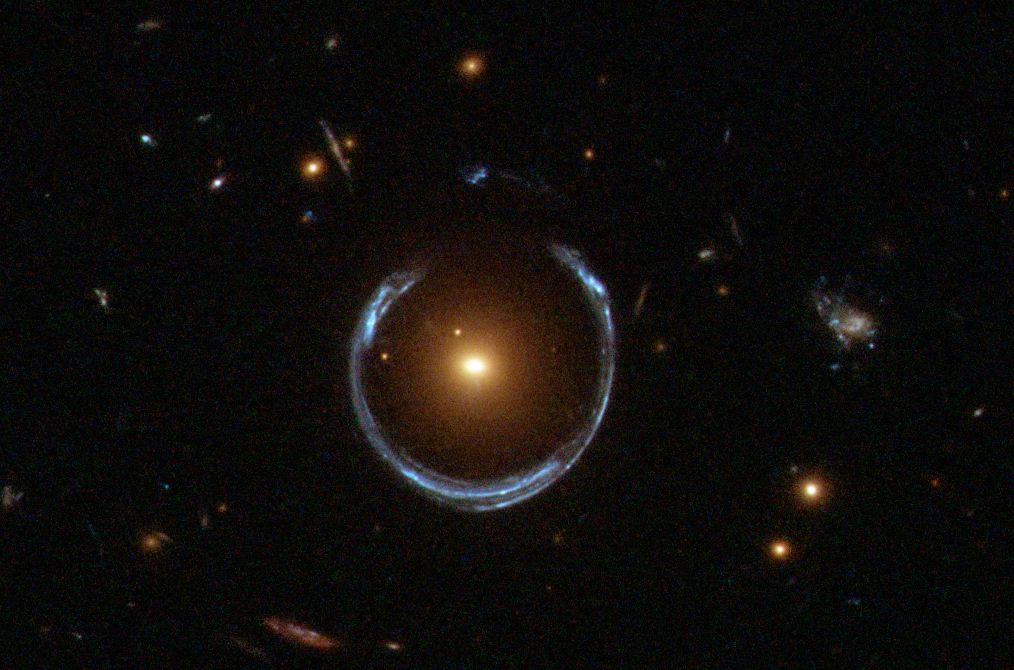
\includegraphics[width = 0.4\textwidth]{img/gravlens2}
\caption{Gravitational lenses are evidence of bent space.}
\label{fig:gravlens}
\end{figure}


Global differential and Riemannian geometry;
Up to now we were looking at arbitrarily small pieces of curves and surfaces. This is local differential geometry.

Global differential geometry deals with manifolds ``in the large''.
Often it connects geometry with topology.


Theorem (Four vertex theorem): Every smooth closed non-self-intersecting curve in the plane has at least for local extrema of curvature.

Theorem (Consequence of Gauss-Bonnet): The torus does not admit metrics with everywhere positive curvature.

Theorem (Geometrization: Thurston-Hamilton-Perelman): Every closed 3-dimensional manifold can be cut into pieces which admit special metrics (most common is the metric of constant negative curvature, the hyperbolic metric).

\end{itemize}



\section{Curves}

\subsection{Parametric Curves}

\begin{defn}
A \emph{Curve} is a trajectory of a point (on the plane or in the space).
\begin{equation*}
\gamma: I \to \mathbb R^2
\end{equation*}
with $I \subset \mathbb R$ being an interval and $\gamma$ continuous.
\end{defn}

There are ``strange'' continuous curves, for example:
\begin{itemize}
\item $\gamma = $ const. $\Rightarrow$ The curve is a point.

\item Peano Curve and Hilbert Curve, which are space-filling curves, i.e.: $\gamma(I) = [0,1]^2 = \blacksquare$.

\item The boundary of the Koch Snowflake.
\end{itemize}


To exclude those, we require differentiability: $C^1$ gives us tangents, $C^2$ gives us curvature, but $C^\infty$ is best.

\begin{defn}
A \emph{smooth parametric curve} in $\mathbb R^n$ is a $C^\infty$-map 
\begin{equation*}
\gamma: I \to \mathbb R^n
\end{equation*}
where $I \subset \mathbb R$ is an interval in $\mathbb R$. Let $t_0 \in I$. The vector 
\begin{equation*}
\dot\gamma(t_0) = \frac{dy}{dt}\Big|_{t = t_0}
\end{equation*}
is called the \emph{velocity vector} of $\gamma$ at $t_0$.
\end{defn}


\begin{figure}[H]
\centering
\def\svgwidth{0.3\textwidth}
\input{img/velocity-vector.pdf_tex}
\caption{Velocity vector in $t_0$}
\label{fig:velocity-vector}
\end{figure}


\begin{defn}
If $\dot\gamma(t_0) = 0$ the $t_0$ is called a \emph{singular point} of $\gamma$. Otherwise $t_0$ is called a \emph{regular point}. If all points are regular, then we call $\gamma$ \emph{regular}.
\end{defn}

\begin{exmp}
Consider the curve
\begin{equation*}
\gamma(t) = (t^3, t^2) \text{ with } I = (-\infty, \infty)
\end{equation*}
Let us search for singularities:
\begin{equation*}
\dot\gamma(t) = (3t^2, 2t) \stackrel{!}{=} (0,0) \Leftrightarrow t = 0
\end{equation*}

\begin{figure}[H]
\centering
\def\svgwidth{0.7\textwidth}
\input{img/cusp.pdf_tex}
\caption{Note the singular point in $(0,0)$. This is called a \emph{cusp}.}
\label{fig:cusp}
\end{figure}
\end{exmp}


\begin{defn}
At a regular point a curve has a \emph{tangent}:

\begin{equation*}
l(t) = \gamma(t_0) + (t-t_0) \cdot \dot\gamma(t_0)
\end{equation*}

This tangent approximates the curve in first order, i.e.:
\begin{equation*}
\gamma(t) = l(t) + o(t-t_0)
\end{equation*}

\end{defn}


\begin{defn}
\emph{Parameter change}: Consider $\gamma: I \to \mathbb R^n$ Let $\phi: J \to I$ where $J$ is another Interval and $\phi$ is a diffeomorphism ($\phi$ bijective and differentiable, $\phi^{-1}$ also differentiable.)

Then, the curve
\begin{equation*}
\delta : J \to \mathbb R^n : s \mapsto \gamma \circ \phi(s)
\end{equation*}
is called a \emph{reparametrization} of $\gamma$.
\end{defn}

\begin{lem}
Regularity is preserved under reparametrization. A point $s_0 \in J$ is a regular point of $\delta$ if and only if $\gamma(s_0)$ is a regular point of $\gamma$.
\end{lem}

\emph{Proof:} By chain rule: 
\begin{equation*}
\dot\delta(s_0) = \dot\gamma(\phi(s_0)) \cdot \phi'(s_0)
\end{equation*}
Since $\phi'(s_0) \neq 0$ because $\phi^{-1}$ is differentiable, one has $\dot\delta(s_0) \neq 0 \Leftrightarrow \dot\gamma(\phi(s_0)) \neq 0$. \hfill $\Box$



\subsection{Length and the natural parameter}

\begin{defn}
Let $\gamma: [a,b] \to \mathbb R^n$ be a smooth curve. Its length is defined as:

\begin{equation*}
\mathcal L(\gamma) = \int_a^b \left\|\gamma\dot(t)\right\| dt
\end{equation*}
\end{defn}

Motivation: $\int_a^b \left\|\gamma\dot(t)\right\| dt $ is the supremum of lengths of inscribed polygons.

\begin{figure}[H]
\centering
\def\svgwidth{0.7\textwidth}
\input{img/inscribed-polygon.pdf_tex}
\caption{A curve and an inscribed polygon.}
\label{fig:inscribed-polygon}
\end{figure}


\begin{lem}
The length of an curve is always longer than the line between the endpoints, i.e.:
\begin{equation*}
\int_{t_i}^{t_{i+1}} \left\|\dot\gamma(t)\right\| dt \geq \left\|\gamma(t_{i+1}) - \gamma(t_i)\right\|
\end{equation*}
\end{lem}
\emph{Proof:} $\int_{t_i}^{t_{i+1}} \left\|\dot\gamma(t)\right\| dt \geq \left\|\int_{t_i}^{t_{i+1}} \dot\gamma(t) dt\right\| =  \left\|\gamma(t_{i+1}) - \gamma(t_i)\right\|$ \hfill $\Box$

\begin{col}
$\mathcal L(\gamma)$ is greater or equal to the length of any inscribed polygon.
\end{col}


\begin{defn}
A curve $\gamma$ is called a \emph{unit-speed curve} if $\forall t : \left\|\dot\gamma(t)\right\| = 1$. For unit-speed curves it holds that $L(\gamma) = b-a$. Unit-speed curves are also called \emph{arc-length parametrizations.}
\end{defn}


\begin{thm}
Every regular curve has a unit-speed reparametrization.
\end{thm}
\emph{Proof:} Let $\gamma: I \to \mathbb R^n$ be regular. Fix $a \in I$ and define
\begin{equation*}
\psi: I \to \mathbb R: t \mapsto \int_a^t \left\|\gamma\dot(s)\right\| ds.
\end{equation*}

Claim: $\psi$ is the inverse of the $\phi$ that we are looking for.
$\psi$ is continuously differentiable: $\psi'(t) = \left\|\dot\gamma(t)\right\| > 0$ and therefore $\psi$ is monotone and $\psi^{-1}$ is also differentiable.
Let $J = \psi(I)$ and $\phi = \psi^{-1}$. One has
\begin{equation*}
\phi'(s) = \frac{1}{\psi'(\phi(s))} = \frac{1}{\left\|\gamma\dot(\phi(s))\right\|}.
\end{equation*}
Therefore: 
\begin{equation*}
\dot\delta(s) = \dot\gamma(\phi(s)) \cdot \phi'(s) = \frac{\dot\gamma(\phi(s))}{\left\|\dot\gamma(\phi(s))\right\|}
\end{equation*}
which is a unit vector. \hfill $\Box$


\begin{defn}
If $\left\|\dot\gamma(t)\right\| = 1$, then $t$ is called a \emph{natural parameter}.

A natural parameter is unique up to starting point and the direction.
\end{defn}


\subsection{Other definitions of a curve}


\begin{obsv}
Let $f: I \to \mathbb R$ be smooth. Then the graph of $f$ can be parameterized: $\gamma(t) = (t, f(t))$. Since the first component never has a derivative of $0$, $\gamma$ is regular.
\end{obsv}

\begin{obsv}
Let $U \subset \mathbb R^2$. Let $F: U \to \mathbb R$ be a smooth function with non-vanishing gradient, i.e. $\nabla F \neq 0$ everywhere.

Then by the Implicit Function Theorem locally $\{(x,y)|F(x,y) = 0\}$ can be represented either as the graph of $y = f(x)$ or $x = f(y)$, therefore it is locally a parametric curve.
\end{obsv}


\begin{exmp}
Consider the circle $\gamma = (cos(t), sin(t))$ or generally closed curves. But what should $I$ be? $[0, 2\pi)$ or $(-\infty, \infty)$
\end{exmp}

\begin{figure}[H]
\centering
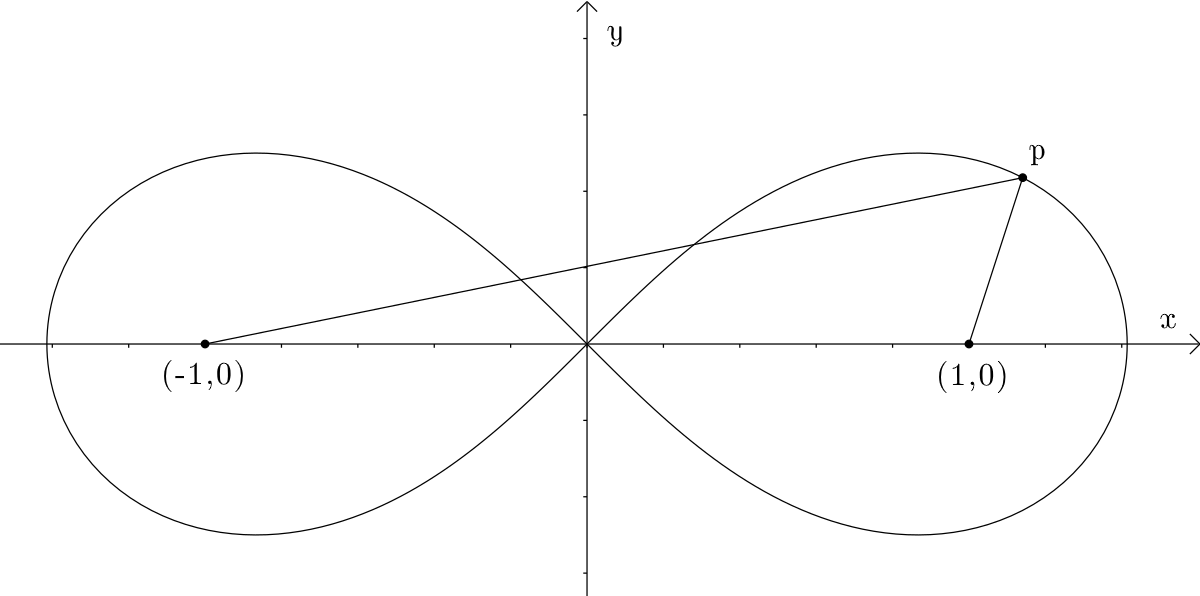
\includegraphics[width = 0.7\textwidth]{img/lemniscate}
\caption{Lemniscate of Bernoulli}
\label{fig:lemniscate}
\end{figure}


\begin{exmp}
Lemniscate of Bernoulli:

Consider the set depicted in Figure \ref{fig:lemniscate}:
\begin{equation*}
\left\{p \in \mathbb R^2 ~|~ dist\left(p, \left(1,0\right)\right) \cdot dist\left(p, \left(-1,0\right)\right) = 1\right\}
\end{equation*}

Is this a curve? Lets look at it from various points of view. The equation from the set above can be rewritten in a more concise from: 
\begin{equation*}
F(x,y) := (x^2+y^2)^2 - 2(x^2-y^2) = 0
\end{equation*}

We can apply the Implicit Function Theorem everywhere except in the point $(0,0)$ since
\begin{equation*}
\nabla F = 0, F = 0 \Leftrightarrow x = 0, y = 0
\end{equation*}

This yields the parametric equations:
\begin{align*}
\gamma_x(t) &= \frac{\sqrt 2 cos(t)}{1+sin^2(t)} \\
\gamma_y(t) &= \frac{\sqrt 2 cos(t) sin(t)}{1+sin^2(t)} \\
\text{with }\forall t:\dot\gamma(t) &\neq 0 
\end{align*}

But what about the point $(0,0)$? This brings us to the following definitions:
\end{exmp}


\begin{defn}
\begin{itemize}
\item The image of a smooth map $I \to \mathbb R^2$ with non-vanishing derivative is called \emph{immersed curve}.

\item A subset of $\mathbb R^2$ which in the neighborhood of every point can be represented as $\{(x,y) ~|~ F(x,y) = 0\}$ with $\nabla F \neq 0$ is called an \emph{embedded curve}.

\item A \emph{generic} immersed curve has no multiple intersections and no self-tangencies. A non-generic curve can be made generic by a small perturbation.
\end{itemize}
\end{defn}

\begin{figure}[H]
\centering
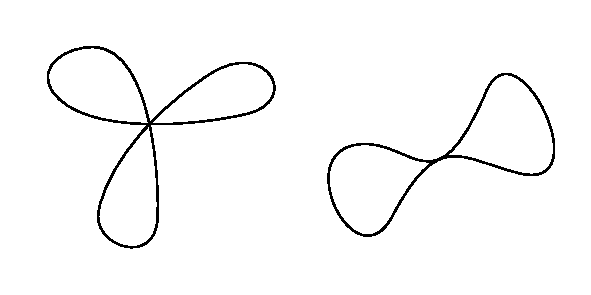
\includegraphics[width = 0.7\textwidth]{img/nongeneric}
\caption{Non-generic Curves: multiple intersection on the left, self-tangency on the right}
\label{fig:non-generic}
\end{figure}


\subsection{Curvature of Curves}

\begin{defn}
Let $\gamma$ be a unit-speed curve in $\mathbb R^n$. Its \emph{curvature} $\kappa(t)$ at the point $\gamma(t)$ is  defined to be $\left\| \ddot\gamma(t)\right\|$. The curvature of an arbitrary regular curve is defined as the curvature of  its unit-speed reparametrization.
\end{defn}

\begin{lem}
A curve has zero curvature everywhere if and only if it is a straight line segment.
\end{lem}
\emph{Proof:} Take the unit-speed reparametrization $\gamma$. Then 
\begin{equation*}
\ddot\gamma(t) = 0 \Leftrightarrow \dot\gamma(t) = \text{const.} \Leftrightarrow \gamma(t) = a\cdot t+b
\end{equation*}
\hfill $\Box$

\begin{lem}
The curvature of a circle of radius $R$ is $\frac{1}{R}$.
\end{lem}

\emph{Proof:} A unit-speed parametrization of the circle is:

\begin{align*}
\gamma(t) &= R \cdot \left(\cos\left(\frac{t}{R}\right), \sin\left(\frac{t}{R}\right)\right) \\
\dot\gamma(t) &= \left(-\sin\left(\frac{t}{R}\right), \cos\left(\frac{t}{R}\right)\right) \\
\ddot\gamma(t) &= -\frac{1}{R} \cdot \left(\cos\left(\frac{t}{R}\right), \sin\left(\frac{t}{R}\right)\right) \\
&\text{thus: } \left\|\ddot\gamma(t)\right\| = \frac{1}{R} 
\end{align*}
\hfill $\Box$

\begin{figure}[H]
\centering
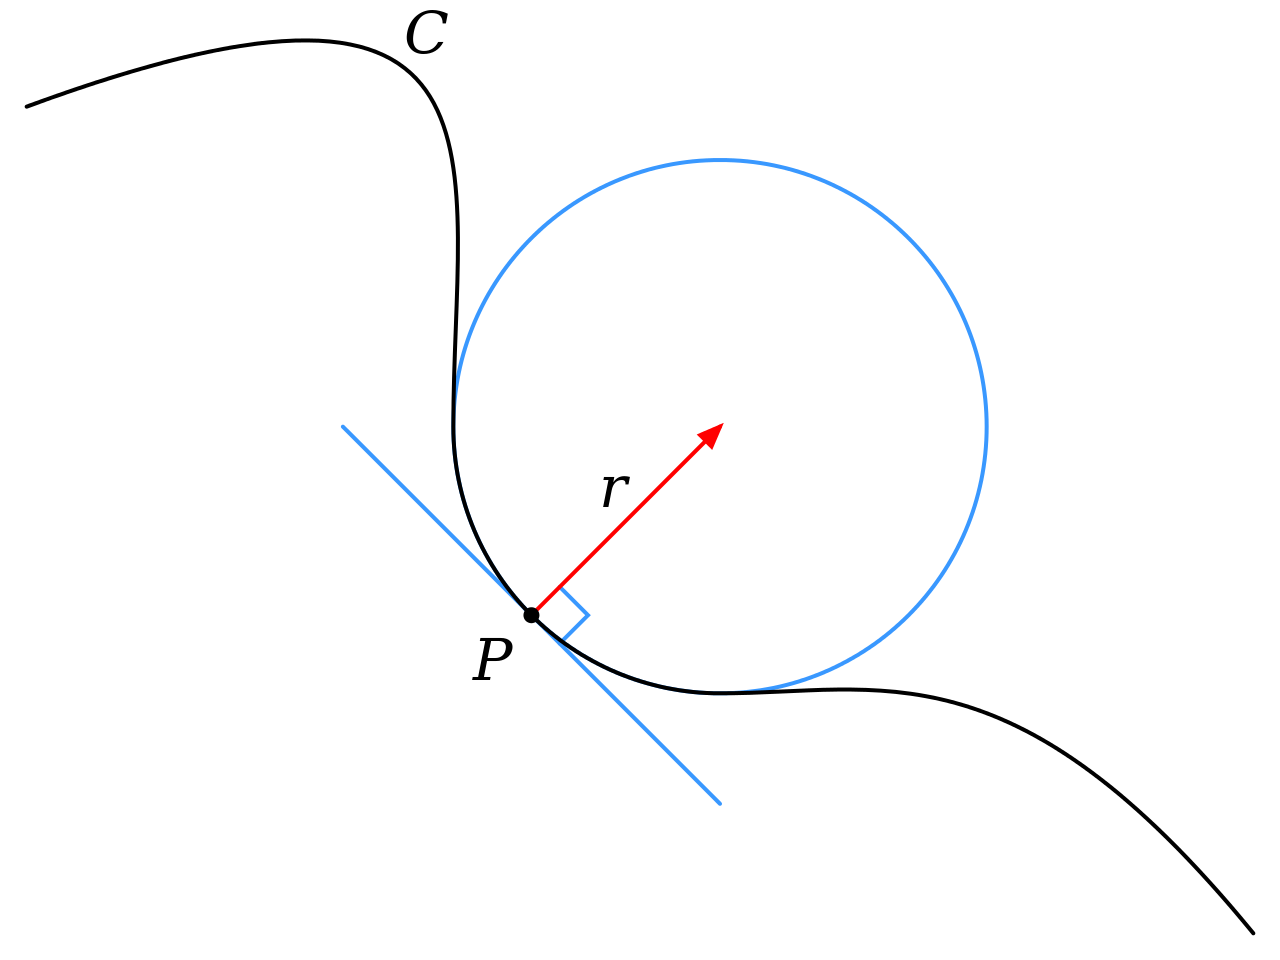
\includegraphics[width = 0.7\textwidth]{img/schmiegekreis}
\caption{A circle touching a curve in a point whose radius is the inverse of the curvature is called \emph{osculating}. It ``snuggles up'' against the curve.}
\label{fig:schmiegekreis}
\end{figure}


To compute the curvature of a non-unit-speed curve, on may use the following Theorem.

\begin{thm}
\label{thm:curvature_arbitrary_curve}
The curvature of an arbitrary regular curve in $\mathbb R^2$ or $\mathbb R^3$ is:

\begin{equation*}
\kappa = \frac{\left\|\dy \times \ddy\right\|}{\left\|\dy\right\|^3}
\end{equation*}

Note: For $a, b \in \mathbb R^2$: $\|a \times b\| := |\det(a~b)|$
\end{thm}

\emph{Proof:} Let $\delta = \gamma \circ \phi$ be a unit-speed reparametrization. By definition:
\begin{equation*}
\kappa(t) = \left\|\ddot\delta(s)\right\|\text{ where }t = \phi(s)
\end{equation*}
Then:
\begin{align*}
\dot\delta(s) &= \dot\gamma\left(\phi(s)\right) \cdot \phi'(s) \\
			  &= \dot\gamma(t) \cdot \phi'(s) \\
\ddot\delta(s) &= \frac{d}{ds} \left(\dot\gamma(t) \cdot \phi'(s)\right) \\
			   &= \ddot\gamma(t) \cdot \left(\phi'(s)\right)^2 + \dot\gamma(t)\phi''(s)
\end{align*}

From this formula we need to eliminate $\phi', \phi''$.

\begin{equation*}
\left\|\dot\delta(s)\right\| = 1 \Rightarrow \phi'(s) = \frac{1}{\left\|\dot\gamma(t)\right\|}
\end{equation*}

Thus:

\begin{align*}
\phi''(s) &= \frac{d}{ds} \frac{1}{\left\|\dot\gamma(t)\right\|} \\
&= \frac{d}{ds} \frac{1}{\sqrt{\left\langle\dot\gamma(t), \dot\gamma(t)\right\rangle}} \\
&= - \frac{1}{2} \frac{1}{\left\langle\dot\gamma(t), \dot\gamma(t)\right\rangle^{3/2}} \frac{d}{ds} \left\langle\dot\gamma(t), \dot\gamma(t)\right\rangle \\
\Big(\text{Using the Leibniz-rule }&\text{for inner products: } \left\langle v,w\right\rangle' = \left\langle v',w\right\rangle + \left\langle v,w'\right\rangle \Big) \\
&= - \frac{1}{2} \frac{1}{\left\|\dot\gamma(t)\right\|^3} \cdot 2 \left\langle\ddot\gamma(t) \phi'(s), \dot\gamma(t)\right\rangle \\
&= - \frac{\left\langle\ddot\gamma(t), \dot\gamma(t)\right\rangle \phi'(s)}{\left\|\dot\gamma\right\|^3} \\
&= - \frac{\left\langle\ddot\gamma(t), \dot\gamma(t)\right\rangle}{\left\|\dot\gamma\right\|^4} \\
\text{Therefore: }\ddot\delta(s) &= \frac{\ddot\gamma}{\left\|\dot\gamma\right\|^2} - \frac{\left\langle\dot\gamma, \ddot\gamma\right\rangle \dot\gamma}{\left\|\dot\gamma\right\|^4} \\
&= \frac{\ddot\gamma \left\langle\dot\gamma, \dot\gamma\right\rangle - \dot\gamma\left\langle\dot\gamma, \ddot\gamma\right\rangle}{\left\|\dot\gamma\right\|^4} \\
\Big(\text{Using the BAC-}& \text{CAB rule } a \times (b\times c) = \left\langle a,c\right\rangle b - \left\langle a,b\right\rangle c \Big) \\
&= \frac{\dot\gamma \times (\ddot\gamma \times \dot\gamma)}{\left\|\dot\gamma\right\|^4}
\end{align*}

Since $\dot\gamma \perp (\ddot\gamma \times \dot\gamma)$, one has 
\begin{equation*}
\left\|\dot\gamma \times (\ddot\gamma \times \dot\gamma)\right\| = \left\|\dot\gamma\right\| \cdot \left\|\ddot\gamma \times \dot\gamma\right\|
\end{equation*}

and therefore 
\begin{equation*}
\left\|\ddot\delta(s)\right\| = \kappa(t) = \frac{\left\|\dy \times \ddy\right\|}{\left\|\dy\right\|^3}
\end{equation*}
\hfill $\Box$


\subsection{Signed curvature and the turning number}

\begin{lem}
If $\gamma$ is a unit-speed curve, then $\ddot\gamma \perp \dot\gamma$.
\end{lem}

\emph{Proof:} $\left\|\dot\gamma\right\| = 1 \Rightarrow \left\langle\dot\gamma, \dot\gamma\right\rangle = 1 \Rightarrow \frac{d}{dt} \left\langle\dot\gamma, \dot\gamma\right\rangle = 0 \Rightarrow 2 \left\langle\ddot\gamma, \dot\gamma\right\rangle = 0 \Rightarrow \dot\gamma \perp \ddot\gamma$ \hfill $\Box$


\begin{figure}[H]
\centering
\def\svgwidth{0.3\textwidth}
\input{img/velocity-and-acceleration.pdf_tex}
\caption{$\ddy$ is also called the \emph{acceleration}.}
\label{fig:velocity-and-acceleration}
\end{figure}


\begin{defn}
Let $\gamma$ be a planar unit-speed curve. Denote by $\nu_s(t)$ (the \emph{signed normal}) the unit vector orthogonal to $\dot\gamma(t)$ such that $(\dot\gamma, \nu_s)$ form a positively oriented ONB (orthonormal basis). The number $\kappa_s(t)$ such that $\ddot\gamma(t) = \kappa_s(t) \nu_s(t)$ is called the \emph{signed curvature} of $\gamma$.
\end{defn}

\begin{obsv}
Clearly, $|\kappa_s(t)| = \kappa(t)$. The sign of $\kappa_s(t)$ indicates the direction of the turn:
\begin{align*}
\kappa_s &< 0\text{: right turn} \\
\kappa_s &> 0\text{: left turn} \\
\kappa_s &= 0\text{: straight}
\end{align*}
An orientation change for $\gamma$ implies a sign change for $\kappa_s(t)$.
\end{obsv}

\begin{defn}
A curve $\gamma : [a,b] \to \mathbb R^n$ is called a \emph{closed regular} curve if the endpoints meet and all derivatives match, i.e.: $\gamma(a) = \gamma(b)$ and $\gamma^{(n)}(a) = \gamma^{(n)}(b)$.
\end{defn}

\begin{thm}
The total signed curvature of a closed regular curve is an integer multiple of $2\pi$:
\begin{equation*}
\int_a^b \kappa_s(t) dt = 2k\pi
\end{equation*}
\end{thm}

For the proof we need an additional Lemma.

\begin{defn}
Let $\dy(t) = (\cos\alpha(t), \sin\alpha(t))$. $\alpha(t)$ is definend up to a summand $2n\pi$. There is a global choice $\alpha: I \mapsto \mathbb R$ such that $\alpha$ is smooth. This function is called the \emph{turning angle}.
\end{defn}

\begin{lem}
$\kappa_s(t) = \dot\alpha(t)$
\end{lem}

\emph{Proof:} $\dy = (\cos \alpha, \sin \alpha)$

$\ddy = (-\sin\alpha, \cos\alpha) \cdot \dot\alpha$

$\nu_s = (-\sin \alpha, \cos \alpha)$

therefore $\kappa_s = \dot\alpha$

\emph{Proof of Theorem:}

$\int_a^b \kappa_s(t) dt = \int_a^b \dot\alpha dt = \alpha(b) - \alpha(a) = 2k\pi$

\hfill $\Box$

\begin{defn}
This number $k$ is called the \emph{turning number} of $\gamma$. It is the number of times the tangent vector rotates when running along the curve.
\end{defn}

\begin{figure}[H]
\centering
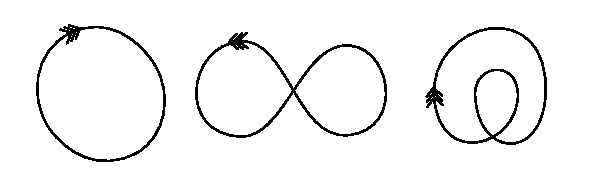
\includegraphics[width = 0.7\textwidth]{img/turning-number-examples}
\caption{Different turning numbers: Circle: $k=1$, Lemniscate: $k=0$, Loop-de-Loop: $k=2$}
\label{fig:turning-number-examples}
\end{figure}

\begin{thm}
(Whitney) The closed planar curves are regularly isotropic if and only if the have the same turning number.

Two curves are \emph{isotropic} if there is a continuous deformation of one curve into the other. Two regular curves are \emph{regularly isotropic} if all intermediate curves are regular as well.
\end{thm}

\emph{Proof:} next time \hfill $\Box$

\begin{figure}[H]
\centering
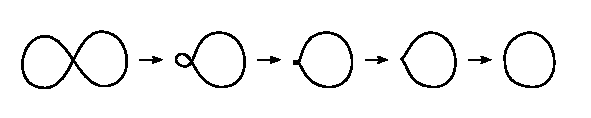
\includegraphics[width = 0.7\textwidth]{img/lemniscate-to-circle}
\caption{The lemniscate and the circle are isotropic but not regularly isotropic. Note the  \emph{cusp} in the fourth step.}
\label{fig:lemniscate-to-circle}
\end{figure}


\begin{thm}
Let $f: I \to \mathbb R$ be any smooth function. Then there is a unit-speed curve $\gamma: I \to \mathbb R^2$ whose singed curvature is f. Besides, $\gamma$ is unique up to a rigid motion: if $\tilde\gamma : I \to \mathbb R^2$ is another unit-speed curve with the signed curvature f, then $\tilde\gamma = M \circ \gamma$ where $M: \mathbb R^2 \to \mathbb R^2$ is a distance and orientation-preserving bijection.
\end{thm}

\emph{Proof:} $\y(t) = y(t_0) + \int_{t_0}^t \dy(t) dt$
$\dy(t) = (\cos\alpha(t), \sin\alpha(t))$
$\dot\alpha(t) = f(t)$

$\y$ has $\kappa_s = f$ if and only if the above equations are satisfied. General solution of the last one:

$\alpha(t) = \alpha(t_0) + \int_{t0}^t f(t) dt$

Then substitue into the second equation, then into the first. Parameters $\alpha(t_0)$ corresponds to rotation and $\y(t_0)$ corresponds to translation, the two free parameters in rigid motion. \hfill $\Box$

\subsection{Space curves: curvature and torsion}

\begin{defn}
Let $\gamma$ be a unit speed curve in $\mathbb R^3$. Denote $\dy(t) =: T(t)$ AS we know, $\left\|\dy\right\| = 1 \Rightarrow \ddy \perp \dy$

Denote $N(t) := \frac{\ddy}{||\ddy||}$ (assuming: $\ddy(t) \neq 0 ~\forall t$)

$N(t)$ is called the \emph{principal normal} of $\gamma$.
\end{defn}

\begin{defn}
The plane through $\gamma(t)$ spanned by $T(t)$ and $N(t)$ is called the \emph{osculating plane}. It has contact of order 2 with $\gamma$, i.e.:

$\gamma(t) = \gamma(t_0) + \dy(t_0)(t-t_0) + \ddy/2(t-t_0)^2 + o((t-t_0)^3)$

The sum of the first 3 terms lies in the osculation plane.
\end{defn}

\begin{defn}
\emph{Torsion} is the turning speed of the osculation plane. (Compare: curvature is the turning speed of the tangent.)
\end{defn}

\begin{defn}
B(t) is the unit vector such that $(T(t), N(t), B(t))$ is a positive ONB. It is called the \emph{binormal} to $\gamma$. The family of bases $(T(t), N(t), B(t))$ is called the \emph{Frenet-Serret frame}. Note that $B(t) = T(t) \times N(t).$
\end{defn}

skizze: FS frame in spiral curve.

\begin{defn-lem}
The derivative of the binormal is collinear with the normal:

$\dot B(t) = -\tau(t) \cdot N(t)$

The number $\tau(t)$ is called the \emph{torsion} of $\gamma$ at $\gamma(t)$

$\tau(t) > 0 \Leftrightarrow$ ``right screw''
\end{defn-lem}

\emph{Proof:} $\left\|B(t)\right\| = 1 \Rightarrow \left\langle\dot B(t), B(t)\right\rangle = 0$. It remains to show $\left\langle\dot B(t), T(t)\right\rangle = 0$.

$B = T \times N$
$\dot B = \dot T \times N + T\times \dot N = \kappa N\times N + T\times \dot N = T\times \dot N \perp T$

\hfill $\Box$

\begin{thm}
Frenet-Serret formulas:
\begin{align*}
\dot T &= \kappa N \\
\dot N &= -\kappa T + \tau B \\
\dot B &= -\tau N
\end{align*}
\end{thm}

\emph{Proof:} The first and the third one hold by definition. The second one:

$\left\langle\dot N, T\right\rangle = -\kappa, \left\langle\dot N, N\right\rangle = 0, \left\langle\dot N, B\right\rangle = \tau$

$\left\langle N, T\right\rangle = 0$ differentiate this:

$<\Dot N, T> + <N, \dot T>$

bla


\begin{lem}
For any regular curve $\y$ in $\mathbb R^3$:
\begin{equation*}
\tau = \frac{det(\dy, \ddy, \dddot\gamma)}{\left\| \dy \times \ddy\right\|^2}
\end{equation*}

In the special case of a unit-speed curve:
\begin{equation*}
\tau = \frac{det(\dy, \ddy, \dddot\gamma)}{\kappa^2}
\end{equation*}

\end{lem}

\emph{Proof:}

Matrix form:

\begin{verbatim}
verbatim just so it compiles right now. todo: stupid matrices
\dot T    (      0 \kappa    0 )   T
\dot N  = (-\kappa      0 \tau ) * N
\dot B    (      0  -\tau    0 )   B
\end{verbatim}

\begin{thm}
Let $(e_1(t), \hdots, e_n(t))$ be a smooth family of ONB in $\mathbb R^n$. Let

$\dot E = Q(t) E$

Then $Q^T(t) = -Q(t)$, i.e.: Q is skew-symmetric.

\end{thm}

\begin{lem}
If $M(t) \in SO(n)$ be a smooth family of orthogonal matrices such that $M(t_0) = I$. Then $\dot M(t_0)$ is skew-symmetric.
\end{lem}

\emph{Proof:} $M^TM = I$, differentiate:

$\dot M^T(t) M(t) + M^T(t) \dot M(t) = 0$

With $t = t_0$: $M(t_0) = I \Rightarrow \dot M(t_0) + \dot M(t_0) = 0$ \hfill $\Box$

\emph{Proof of Theorem:} 

Notation $\mathcal E(t) = e...e$

Let $\mathcal E(t) = M(t)\cdot\mathcal E(t_0)$, $M(t) \in \mathbb R^{n\times n}$

Besides, $M(t) \in SO(n), M(t_0) = I$

Using the Lemma we get $\dot M(t_0)$ is skew-symmetric.

$\mathcal E(t_0) = Q(t_0) \cdot \mathcal E(t_0)$

bla bla \hfill $\Box$


\begin{thm}
Let $f: I\to \mathbb R, g: I \to \mathbb R$ be smooth functions with $f(t) > 0 ~\forall t.$ Then there is a unique up to a rigid motion unit-speed curve $\gamma: I \to \mathbb R^3$ with curvature f and torsion g.
\end{thm}

\emph{Sketch of Proof:} It is basically solving a vector-valued ODE:
\begin{equation*}
bla, nachher
\end{equation*}

It has a unique solution for any initial data $(T(t_0), N(t_0), B(t_0))$. Put $\gamma(t) = \dy(t_0) + \int_{t_0}^t T(t) dt$. Then $(T, N, B)$ is the Frenet-Surret frame for $\gamma$. B is the binormal, because the solution of the above ODE is an ONB.

\hfill $\Box$

\begin{thm}
(Fenchel:) The total curvature of a closed space curve is:
\begin{equation*}
\int_a^b \kappa(t) dt \leq 2\pi
\end{equation*}

It is equal to $2\pi$ if and only if the curve is planar and convex.

\end{thm}

\begin{lem}
\begin{equation*}
\int_a^b \kappa(t) dt = L(T)
\end{equation*}
where $T:[a,b] \to \mathcal S^2 \subset \mathbb R^3$ is the \emph{tangent indicatrix}.
\end{lem}

\begin{lem}
$T$ is contained in a great circle if and only if $\gamma$ is planar.
\end{lem}

\begin{lem}
$T$ intersects every great circle at least once.
\end{lem}

\begin{thm}
(Crofton:) Length of a spherical curve is half of the integral of the number of its intersections with great circles.
\end{thm}





\section{Exercises}

\subsection{Exercise 1}

\begin{enumerate}

\item
\begin{enumerate}
\item \emph{Show that every tangent to the parabola $y=x^2$ is perpendicular to the line through the focus $F := (0, \frac{1}{4})$ and the intersection point of the tangent with the $x$-axis.}

Let $K := (k, 0)$ be the intersection point of the tangent with the $x$-Axis and let $P := (p, p^2)$ be the point where the  tangent touches the parabola. Let us find a connection between $k$ and $p$. The slope of the tangent on the one hand is known by the derivative of the parabola at $p$ and on the other hand is known by the slope triangle formed by $K$, $P$ and $(p,0)$. Thus it must hold that:

\begin{equation*}
2p = \frac{p^2}{p-k}
\end{equation*}

Rearranging this equation gives us our desired connection:

\begin{equation*}
p = 2k
\end{equation*}

Now, with this knowledge we can take the dot-product of $\overrightarrow{KP} = (p-k, p^2) = (k, 4k^2)$ and $\overrightarrow{KF} = (-k, \frac{1}{4})$.

\begin{equation*}
\overrightarrow{KP} \cdot \overrightarrow{KF} = -k^2 + \frac{4}{4}k^2 = 0
\end{equation*}

Thus, the tangent and the focal line are indeed perpendicular. \hfill $\Box$

\item \emph{Show that if two tangents meet on the directrix $y = -\frac{1}{4}$, then they are perpendicular.}

Let $a$ and $b$ be tangent points of the parabola. We then have the following tangent equations:
\begin{align*}
	t_a(x)&=2a\cdot (x-a)+a^2\\
	t_b(x)&=2b\cdot (x-b)+b^2
\end{align*}
For the scalar product of the tangent vectors we have
\begin{equation*}
\begin{pmatrix}
1 \\ 2a\end{pmatrix} \cdot \begin{pmatrix} 1 \\ 2b\end{pmatrix}=4ab-1
\end{equation*}
We thus have to show that $4ab-1=0$.

Since both tangents should meet on the directrix we have
\begin{align*}
	2a(x-a)+a^2&=-\frac{1}{4} \Leftrightarrow x=-\frac{1}{8a}+\frac{a}{2} \\
	2b(x-b)+b^2&=-\frac{1}{4} \Leftrightarrow x=-\frac{1}{8b}+\frac{b}{2}\\
\end{align*}
as well as
\begin{equation*}
	-\frac{1}{8a}+\frac{a}{2} = -\frac{1}{8b}+\frac{b}{2} \Leftrightarrow 4ab-1=0
\end{equation*}
\end{enumerate}

\item \emph{Compute the length of one arc of the cycloid.}

This is a simple integral using a rather rare trig identity, which however can be easily derived from the more common one: $\sin(t)^2 = \frac{1}{2} - \frac{1}{2}\cos(2t)$.
\begin{align*}
\mathcal L(\gamma) &= \int_0^{2\pi} \left\| \dot\gamma \right\| dt \\
&= \int_0^{2\pi} \sqrt{(1-\cos(t))^2 + \sin(t)^2} dt \\
&= \int_0^{2\pi} \sqrt{1 - 2\cos(t) + \cos(t)^2 + \sin(t)^2} dt \\
&= \int_0^{2\pi} \sqrt{2 - 2\cos(t)} dt \\
&= \int_0^{2\pi} 2 \sin\left(\frac{t}{2}\right) dt \\
&= 2 \cdot 2 \cos\left(\frac{t}{2}\right)\Bigg|_0^{2\pi} = 8
\end{align*}
\hfill $\Box$

\item \emph{Compute the curvature of the cycloid at each point. How does the curvature behave near the singular points?}

This is best done by referencing Theorem \ref{thm:curvature_arbitrary_curve}.

\begin{align*}
\kappa(t) &= \frac{\left\|\dy \times \ddy\right\|}{\left\|\dy\right\|^3} \\
&= \frac{|\cos(t) - \cos(t)^2 - \sin(t)^2|}{(2 - 2\cos(t))^{\frac{3}{2}}} \\
&= \frac{1}{2^{\frac{3}{2}}} \frac{1 - \cos(t)}{(1 - \cos(t))^{\frac{3}{2}}} \\
&= \frac{1}{2^{\frac{3}{2}}} \frac{1}{\sqrt{1 - \cos(t)}}
\end{align*}

Note that as $t$ approaches a multiple of $2\pi$, where the singular points are located, the denominator tends to $0$ and thus the curvature approaches $\infty$.



\item \emph{Show that the perimeter of the ellipse with half-axes $a>b$ is equal to }

\begin{equation*}
4a \int_0^\frac{\pi}{2} \sqrt{1 - k^2 \sin^2t} ~dt = 4a \int_0^1 \frac{\sqrt{1 - k^2 x^2}}{\sqrt{1 - x^2}} ~dx
\end{equation*}

\emph{where $k = \sqrt{1 - \frac{b^2}{a^2}}$ is the eccentricity of the ellipse. (This integral is called the complete elliptic integral of the second kind.)}

We will consider only the upper right quarter of the ellipse, but count it 4 times because of symmetry. Consider the parametrization $\gamma(t) = (a \sin(t), b \cos(t))$ for $t \in (0, \frac{\pi}{2})$.

\begin{align*}
4 \mathcal L(\gamma) &= 4 \int_0^\frac{\pi}{2} \sqrt{a^2 \cos^2t + b^2\sin^2t} ~dt \\
&= 4a \int_0^\frac{\pi}{2} \sqrt{\cos^2t + \frac{b^2}{a^2}\sin^2t} ~dt \\
&= 4a \int_0^\frac{\pi}{2} \sqrt{1 - \left(1 - \frac{b^2}{a^2}\right)\sin^2t} ~dt \\
&= 4a \int_0^\frac{\pi}{2} \sqrt{1 - k^2 \sin^2t} ~dt 
\end{align*}

Using the substitution $x = sin(t)$ with $dt = \frac{1}{\sqrt{1-x^2}} ~dx$ we get our result. Note that the fact that the parameter space is only $(0, \frac{\pi}{2})$ is important now, as $\sin(t)$ has to be monotonic in the interval for the substitution to be legal. 

\begin{align*}
4 \mathcal L(\gamma) &= 4a \int_0^1 \frac{\sqrt{1 - k^2 x^2}}{\sqrt{1 - x^2}} ~dx
\end{align*}

\hfill $\Box$

\end{enumerate}

\section{Copy-Paste-Quellen}


%umgebungen

\begin{thm}

\end{thm}
\emph{Proof:} trivial \hfill $\Box$

\begin{lem}

\end{lem}
\emph{Proof:} trivial \hfill $\Box$


\begin{exmp}

\end{exmp}


\begin{defn}

\end{defn}


%equations

\begin{equation}
x = y
\end{equation}


\begin{equation*}
x = y
\end{equation*}


\begin{align}
a &= b \\
c &= d + e
\end{align}


\begin{align*}
a &= b \\
c &= d + e
\end{align*}





%\bibliography{lit}
%\bibliographystyle{plain}
\end{document}

